
%%%%%%%%%%%%%%%%%%%%%%%%%%%%%%%%%%%%%%%%%%%%%%%%%%%%%%%%%%%%%%%%%%%%%%%%%%%%%%%%%%%%%%%
%%%%%%%%%%%%%%%%%%%%%%%%%%%%%%%%%%%%%%%%%%%%%%%%%%%%%%%%%%%%%%%%%%%%%%%%%%%%%%%%%%%%%%%
% 
% This top part of the document is called the 'preamble'.  Modify it with caution!
%
% The real document starts below where it says 'The main document starts here'.

\documentclass[12pt]{article}

\usepackage{amssymb,amsmath,amsthm}
\usepackage[top=1in, bottom=1in, left=1.25in, right=1.25in]{geometry}
\usepackage{fancyhdr}
\usepackage{enumerate}
\usepackage{listings}
\usepackage{graphicx}
\usepackage{float}

\usepackage{mwe}
\usepackage{caption}
\usepackage{subcaption}
% Comment the following line to use TeX's default font of Computer Modern.
\usepackage{times,txfonts}



\makeatletter
\renewcommand*\env@matrix[1][*\c@MaxMatrixCols c]{%
  \hskip -\arraycolsep
  \let\@ifnextchar\new@ifnextchar
  \array{#1}}
\makeatother

\newtheoremstyle{homework}% name of the style to be used
  {18pt}% measure of space to leave above the theorem. E.g.: 3pt
  {12pt}% measure of space to leave below the theorem. E.g.: 3pt
  {}% name of font to use in the body of the theorem
  {}% measure of space to indent
  {\bfseries}% name of head font
  {:}% punctuation between head and body
  {2ex}% space after theorem head; " " = normal interword space
  {}% Manually specify head
\theoremstyle{homework} 

% Set up an Exercise environment and a Solution label.
\newtheorem*{exercisecore}{Exercise \@currentlabel}
\newenvironment{exercise}[1]
{\def\@currentlabel{#1}\exercisecore}
{\endexercisecore}

\newcommand{\localhead}[1]{\par\smallskip\noindent\textbf{#1}\nobreak\\}%
\newcommand\solution{\localhead{Solution:}}

%%%%%%%%%%%%%%%%%%%%%%%%%%%%%%%%%%%%%%%%%%%%%%%%%%%%%%%%%%%%%%%%%%%%%%%%
%
% Stuff for getting the name/document date/title across the header
\makeatletter
\RequirePackage{fancyhdr}
\pagestyle{fancy}
\fancyfoot[C]{\ifnum \value{page} > 1\relax\thepage\fi}
\fancyhead[L]{\ifx\@doclabel\@empty\else\@doclabel\fi}
\fancyhead[C]{\ifx\@docdate\@empty\else\@docdate\fi}
\fancyhead[R]{\ifx\@docauthor\@empty\else\@docauthor\fi}
\headheight 15pt

\def\doclabel#1{\gdef\@doclabel{#1}}
\doclabel{Use {\tt\textbackslash doclabel\{MY LABEL\}}.}
\def\docdate#1{\gdef\@docdate{#1}}
\docdate{Use {\tt\textbackslash docdate\{MY DATE\}}.}
\def\docauthor#1{\gdef\@docauthor{#1}}
\docauthor{Use {\tt\textbackslash docauthor\{MY NAME\}}.}
\makeatother

% Shortcuts for blackboard bold number sets (reals, integers, etc.)
\newcommand{\Reals}{\ensuremath{\mathbb R}}
\newcommand{\Nats}{\ensuremath{\mathbb N}}
\newcommand{\Ints}{\ensuremath{\mathbb Z}}
\newcommand{\Rats}{\ensuremath{\mathbb Q}}
\newcommand{\Cplx}{\ensuremath{\mathbb C}}
%% Some equivalents that some people may prefer.
\let\RR\Reals
\let\NN\Nats
\let\II\Ints
\let\CC\Cplx
%%%%%%%%%%%%%%%%%%%%%%%%%%%%%%%%%%%%%%%%%%%%%%%%%%%%%%%%%%%%%%%%%%%%%%%%%%%%%%%%%%%%%%%
%%%%%%%%%%%%%%%%%%%%%%%%%%%%%%%%%%%%%%%%%%%%%%%%%%%%%%%%%%%%%%%%%%%%%%%%%%%%%%%%%%%%%%%
% 
% The main document start here.

% The following commands set up the material that appears in the header.




%  \textbf{Code:}
%  \begin{center}
%  \lstinputlisting[basicstyle = \footnotesize]{}
%  \end{center}
%  
%  \begin{footnotesize}
%  \begin{verbatim}
%    
%  \end{verbatim}
%  \end{footnotesize}
%  
%  
%  \begin{figure}[H]
%    \begin{center}
%      \caption{}
%    \includegraphics[width = \textwidth]{}
%    \end{center}
%  \end{figure}




\doclabel{Stat 461: Homework 5}
\docauthor{Stefano Fochesatto}
\docdate{February 23, 2022}

\begin{document}
\begin{exercise}{1} Here are some data where the observations are divided into an $x$ group and a $y$ group. 
  \begin{footnotesize}
  \begin{verbatim}
  data_mat <-structure(c(4, 5, 9, 10, 6, 4, 13, 4, 16, 14, 9, 2, 7, 6,
  9, 16, 7, 7, 7, 9, 1, 15, 11, 20, 8, 5, 19, 16, 17, 18, 18, 18, 17,
  20, 15, 29, 16, 14, 17, 17, 25, 17, 1, 12, 33, 26, 16, 3, 25, 7, 2,
  30, 16, 24, 6, 3, 23, 24, 24, 15, 2.02, 3.54, 2.27, 4.97, 4.2, 3.15,
  4.07, 3.3, 4.2, 4.55, 5.3, 3.86, 4.44, 5.65, 3.23, 6.4, 3.61, 4.63,
  4.34, 3.58, 2.13, 5.1, 4.43, 5, 2.46, 2.77, 3.67, 5.67, 5.26, 5.03,
  3.25, 5.21, 2.85, 3.87, 4.57, 4.79, 4.17, 4.91, 3.5, 3.42, 3.86, 3.45,
  4.73, 2.77, 2.76, 2.67, 4.09, 3.46, 4.03, 3.23, 2.64, 5.92, 4.54, 3.55,
  3.43, 4.2, 3.88, 3.59, 3.48, 5.66, 2.48, 6.57, 7.52, 11.47, 6.26, 4.83,
  7.6, 9.54, 11.35, 9.96, 10, 7.4, 5.58, 8.91, 8.64, 10.77, 6.04, 9.28, 8.47,
  5.72), .Dim = c(20L, 7L), .Dimnames = list(NULL, c("y1", "y2", "y3", "x1", "x2", "x3", "x4")))
  \end{verbatim}
  \end{footnotesize}
  \begin{enumerate}
    \item[a.] Using R, run the Mantel test to see if the distance structure in y1, y2, y3 (count data) is the same as 
    the distance structure for the x1, x2, x3, x4 data.\\
    \solution Before we can compute a Mantel test, we must first obtain a distance measure for each group. In the examples that were shown in class 
    we standardized each variable then computed the euclidean distance between each observation (We will also test the count data with the Bray-Curtis measure using the vegan package). 
    Proceeding similarly we get a p-value of 0.0002, so at 
    the $\alpha = .05$  level we would reject the null and conclude that the distance measures for each group are correlated, ie they cluster in a similar way. 
    Plotting the null distribution, and double checking our mantel test with the mantel() function from the vegan package we get the same conclusion,\\ 
    \textbf{Code:}
    \begin{center}
    \lstinputlisting[basicstyle = \footnotesize]{r1.txt}
    \end{center} 
      \begin{figure}[H]
        \begin{center}
          \caption{Distribution of test statistic under the null.}
        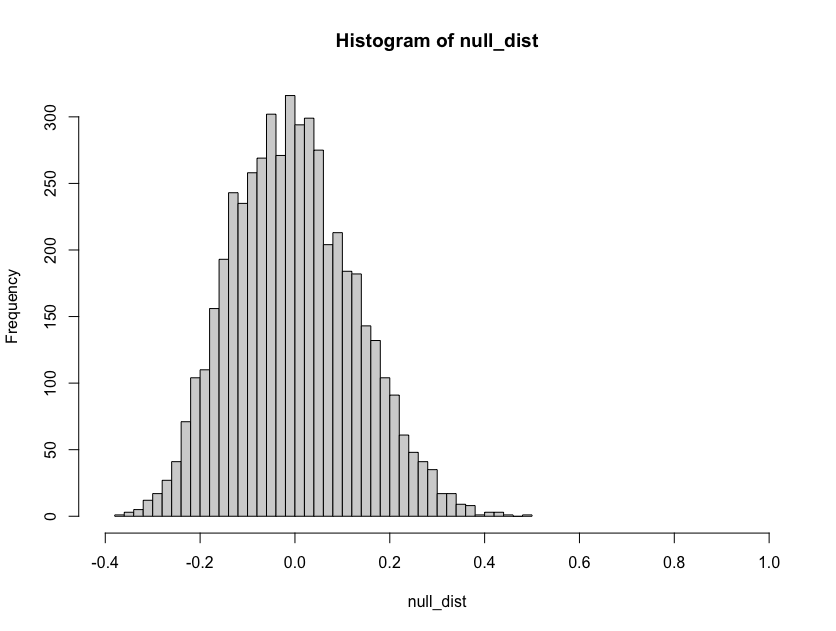
\includegraphics[width = \textwidth]{Rplot.png}
        \end{center}
      \end{figure}
    \vspace{.15in}
    

    \item[b.] What are your conclusions? what does the Mantel test actually test? What is the null hypothesis?\\
    \solution Like we previously stated, we conclude that the groups have correlated distance measures we can also sat that the groups 
    cluster in a similar way. The null of the Mantel test assumes that the distance measures are uncorrelated, the alternative states that they 
    are correlated. When we do a randomization test, we sample the distribution of the test statistic under the assumption of the null hypothesis since 
    distances should be uncorrelated when the order of observations in  one of the groups is randomized. With that sample distribution and our original test 
    statistic we can compute a p-value. 
  \end{enumerate}
\end{exercise}
\vspace{1in}





\begin{exercise}{2} The following is a phylogenetic distance matrix. Use multidimensional scaling (metric, that is , cmdscale) to make a map 
  of these species. What does it mean?
    \begin{footnotesize}
    \begin{verbatim}
    HomoSapiens      0.000 0.089 0.104 0.161 0.182 0.232 0.233 0.249 0.256 0.273 0.322 0.308
    Pan              0.089 0.000 0.106 0.171 0.189 0.243 0.251 0.268 0.249 0.284 0.321 0.309
    Gorilla          0.104 0.106 0.000 0.166 0.189 0.237 0.235 0.262 0.244 0.271 0.314 0.293
    Pongo            0.161 0.171 0.166 0.000 0.188 0.244 0.247 0.262 0.241 0.284 0.303 0.293
    Hylobates        0.182 0.189 0.189 0.188 0.000 0.247 0.239 0.257 0.242 0.269 0.309 0.296
    MacacaFuscata    0.232 0.243 0.237 0.244 0.247 0.000 0.036 0.084 0.124 0.289 0.314 0.282
    MacacaMulatta    0.233 0.251 0.235 0.247 0.239 0.036 0.000 0.093 0.120 0.293 0.316 0.289
    MacacaFascicular 0.249 0.268 0.262 0.262 0.257 0.084 0.093 0.000 0.123 0.287 0.311 0.298
    MacacaSylvanus   0.256 0.249 0.244 0.241 0.242 0.124 0.120 0.123 0.000 0.287 0.319 0.287
    SaimiriSciureus  0.273 0.284 0.271 0.284 0.269 0.289 0.293 0.287 0.287 0.000 0.320 0.285
    TarsiusSyrichta  0.322 0.321 0.314 0.303 0.309 0.314 0.316 0.311 0.319 0.320 0.000 0.252
    LemurCatta       0.308 0.309 0.293 0.293 0.296 0.282 0.289 0.298 0.287 0.285 0.252 0.000
      \end{verbatim}
    \end{footnotesize}
    \solution Running the multidimensional scaling function cmd scale we get the following plot of each of the observations. \\
    \textbf{Code:}
    \begin{center}
    \lstinputlisting[basicstyle = \footnotesize]{r2.txt}
    \end{center} 

    \begin{figure}[H]
      \begin{center}
        \caption{MDS plot of phylogenetic distance matrix.}
      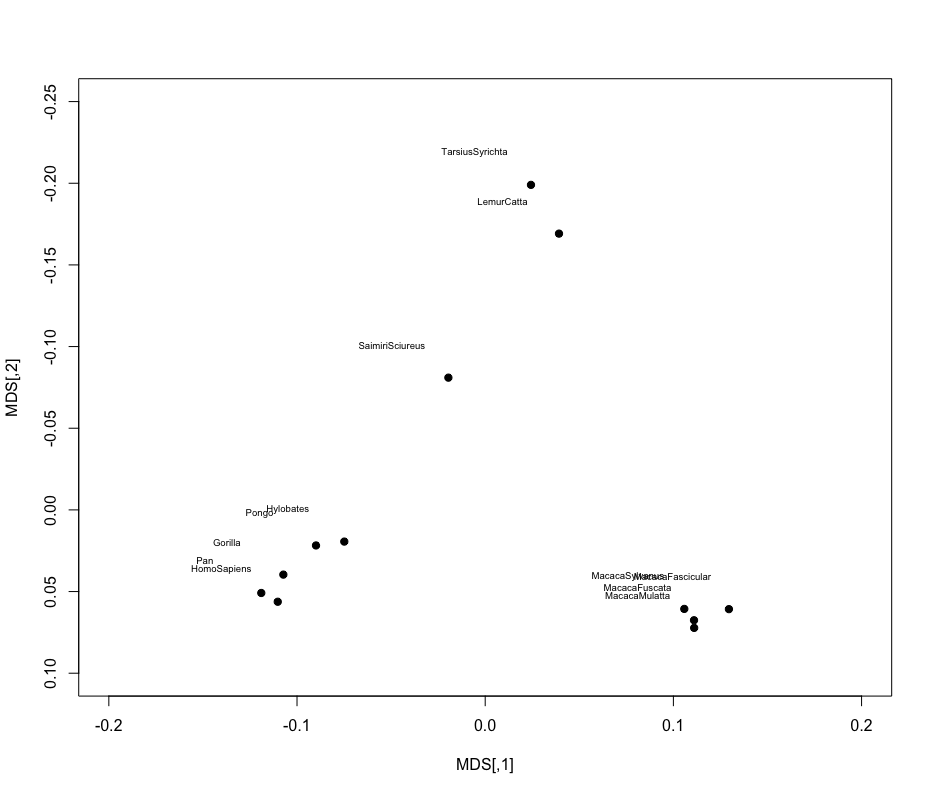
\includegraphics[width = \textwidth]{Rplot01.png}
      \end{center}
    \end{figure}


    We can see some obvious clustering going on in 2-dimensions. The bottom left corner contains larger primates like Gorilla, Homosapians, Pan and Pongo. 
    the bottom right we can see a clustering of different species in the Macaca genus. The upper cluster seem to be smaller primates like Lemurs and Trasius. 
    When we look at the GOF of our multidimensional scaling we see that we kept around 59\% of the variance after compressing the dimension. It might be worthwhile to explore
    visualizing the data in three dimensions, because when we look at the GOF in three dimensions we get around 73\% of the variance. Doing so we get the following plot, 
    \begin{figure}[H]
      \begin{center}
        \caption{MDS plot of phylogenetic distance matrix with 3 dimensions.}
      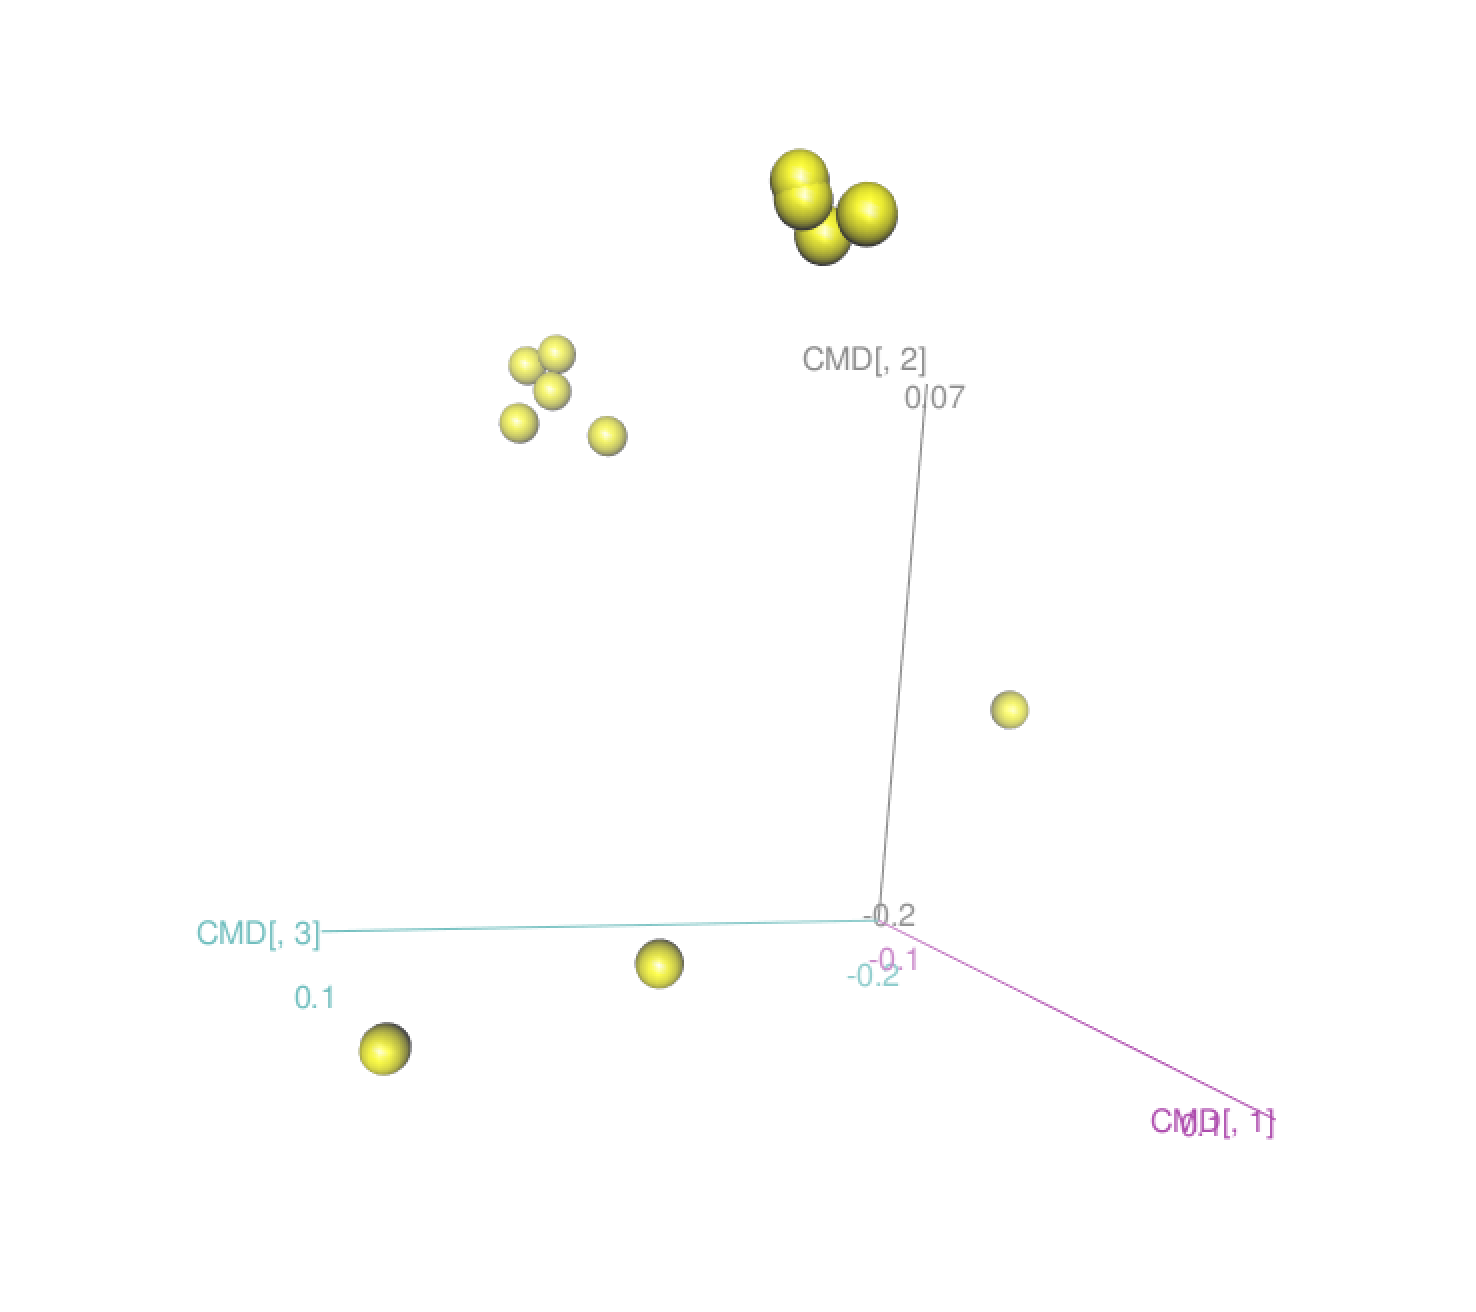
\includegraphics[width = \textwidth]{Rplot02.png}
      \end{center}
    \end{figure}
    This shows us that the lower group of observations isn't really a cluster. It's possible that in higher dimensions there is a greater distance among the group of large primates, I would assume because of 
    the relation in genus the other cluster stays relatively close together in higher dimensions.  
\end{exercise}
\vspace{1in}






\begin{exercise}{3} Using the R base function princomp() does principal component analysis. Run the following.\\
  \begin{footnotesize}
    \begin{verbatim}
      X <- data_mat[,4:7]
      summary(X)
      pairs(X)
      #
      #
      tmp <- princomp(X) 
      plot(tmp)
      tmp
      summary(tmp)
      #
      tmp2 <- princomp(X, cor=TRUE)
      plot(tmp2)tmp2summary(tmp2)
    \end{verbatim}
  \end{footnotesize}
  \begin{enumerate}
    \item[a.] Does using cor=TRUE make a difference? In general, when should you not use cor=TRUE? When should you use cor=TRUE? Try 
    multiplying column x1 by 100 and run princomp() both ways. Does this support your thoughts about correlation vs covariance matrices in principal components?\\
    \solution Yes, using the correlation matrix for principal component analysis removes the effect of scale for all of the variables, essentially standardizing each variable. 
    If the scale matters in our analysis then we would want to use the covariance matrix. If scale doesn't matter then the correlation matrix is suitable and even better conditioned for 
    the eigenvalue problem. Beyond that if you have a constant variable, the variance will be 0 and the related correlations will be undefined.\\\\
    Running the following code we see this in action. When we scale the first variable by 100 our covariance matrix PCA attributes all the variance in the data to that first variable. While the 
    correlation matrix PCA is invariant to change in scale.\\
    \textbf{Code:}
    \begin{center}
    \lstinputlisting[basicstyle = \footnotesize]{r3.txt}
    \end{center} 
    \vspace{.15in}

    \item[b.] Looking at the variances (for instance, when cor=TRUE), how many principal components do you think you should use? Why? Does it look 
    like principal components was a good approach to follow in this case, why or why not?\\
    \solution It seems as though there are several rule of thumb test to decide how many components we should retain. I've hear we include them from largest to smallest until we've explained 80\% of the 
    variance. I've heard the same rule for 90\% and I've also heard that you should drop any components that contribute less than 10\% to the variance. I think that looking at our data it seems as though we only need to 
    retain 3 of the 4 components.\\\\
    I like to think of the components as the magnitude of the semi-axis of the hyperellipse which bounds the data. When we have a small value for a component there exists a hyperellipse in a smaller dimension which is a good approximation for the larger dimension.
    Generally when we have small components in our data, we are adding extra unneeded complexity(both computationally, and parsimoniously) in the form of another dimension. Whenever we can effectively reduce the dimension of our data with PCA, it is worthwhile. 
    \vspace{.15in}
    
    \item[c.] What does the following set of loadings and scores tell you (in general, what are loadings and scores and what are they used for)?\\
    \begin{footnotesize}
      \begin{verbatim}
        X <- data_mat[,4:7]
        hold = princomp(X, cor=TRUE, scores=TRUE)
        names(hold)
        hold$scores
        hold$loadings
      \end{verbatim}
    \end{footnotesize}
    \solution Running the given code we get the following loadings and scores. \\
    \textbf{Code:}
    \begin{center}
    \lstinputlisting[basicstyle = \footnotesize]{r4.txt}
    \end{center}
    The loadings tell us how much of each variable should be weighted when computing the component, and the scores tell us the weight of each component in a given observation. 
    \vspace{.15in}


    \item[d.] Repeat a (correlation-based) principal component analysis on the following. What conclusions do you draw? Do the variances 
    of the principal components add up to 4 (which is the number of variables)?\\
    \begin{footnotesize}
      \begin{verbatim}
        M <-structure(c(-1.4, -1.09, -0.19, -0.09, 1.04, -0.5, -0.22, -1.65, -1.02,
        0.71, 0.23, -0.48, -1.4, -1.2, -0.5, 0.19, 0.9, -0.59, -0.23, -1.9, -0.73,
        0.84, 0.21, -0.46, -1.62, -1.02, 0.03, 0.18, 1.11, -0.62, -0.12, -1.45, -1.13,
        0.93, 0.4, -0.52, -1.52, -1.11, -0.24, -0.9, 0.99, -0.38, -0.04, -1.54, -1.15,
        0.37, 0.48, -0.35), 
        .Dim = c(12L, 4L), .Dimnames = list(NULL, c("X1", "X2", "X3", "X4")))
      \end{verbatim}
    \end{footnotesize}
    \solution Running the correlation-based PCA we get the following,\\
    \textbf{Code:}
    \begin{center}
    \lstinputlisting[basicstyle = \footnotesize]{r5.txt}
    \end{center}
    Looking at the proportion of variance explained it seems clear the the data are highly one dimensional since we used the correlation based approach we 
    can be sure that this behavior is not due to variable scaling.  I would likely conclude that the data could be successfully reduced to a single dimension
    with a very little drop in variance. 
  \end{enumerate}
\end{exercise}
\vspace{1in}







\begin{exercise}{4} Find any multivariate data set of interest to you and perform PCA. The data should have at least three columns. Did PCA help to reduce 
  dimensionality? Looking at the loadings of PC1, what does the PC seem to represent? Try to find a data set that (as far as you can tell) has not already had PCA
  performed on it online?\\
  \solution The data set I used comes from a survey of couples on the subject of their relationship with the goal building a model to predict if the couple is divorced or not. The data set has
  54 predictors which represent survey questions with participants responding on an integer scale from 0 to 4. The data was downloaded from UC Irvine open source machine learning data repository.
  Performing a PCA(covariance based) using princomp() we find that almost 77\% of the variance is explained by a single component. Looking at the loadings for that component it seems to represent a fairly
  even weighted sum, with only survey questions 6 and 7 contributing noticeably less than the others.\\
  \textbf{Code:}
  \begin{center}
  \lstinputlisting[basicstyle = \footnotesize]{r6.txt}
  \end{center} 
  \begin{figure}[H]
    \begin{center}
      \caption{Bar plot of Loadings for each question in the survey.}
    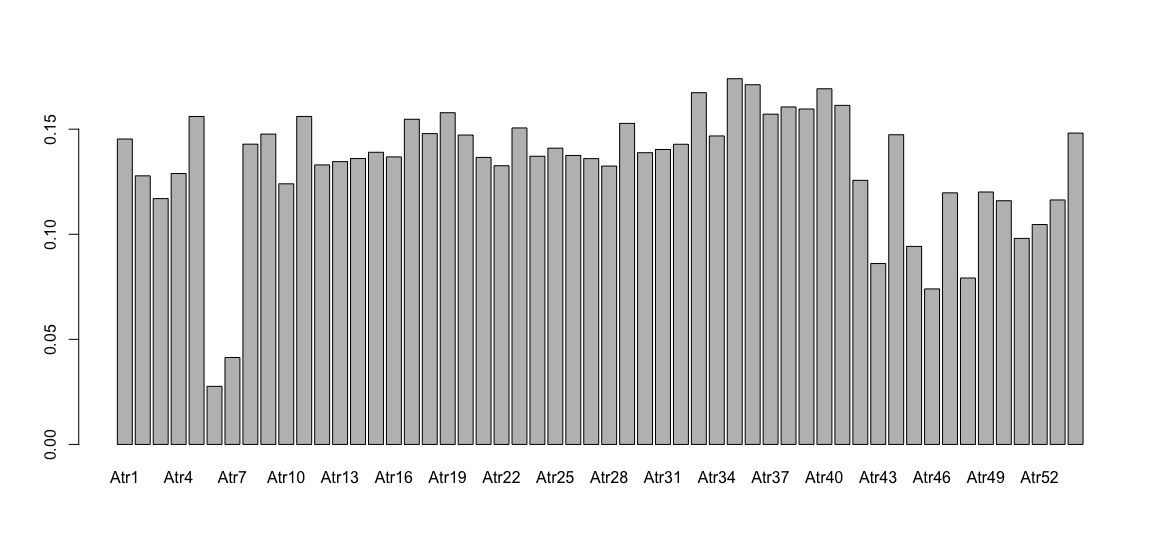
\includegraphics[width = \textwidth]{Rplot03.png}
    \end{center}
  \end{figure}



  Looking at the scores of the observations in the first component we see they exhibit clear bimodalness, where the boundary seems to designate the divorced and non-divorced observations (around observation 85).

  \textbf{Code:}
  \begin{center}
  \lstinputlisting[basicstyle = \footnotesize]{r7.txt}
  \end{center} 
  \begin{figure}[H]
    \begin{center}
      \caption{Histogram of Scores in the first component for each participant in the survey.}
    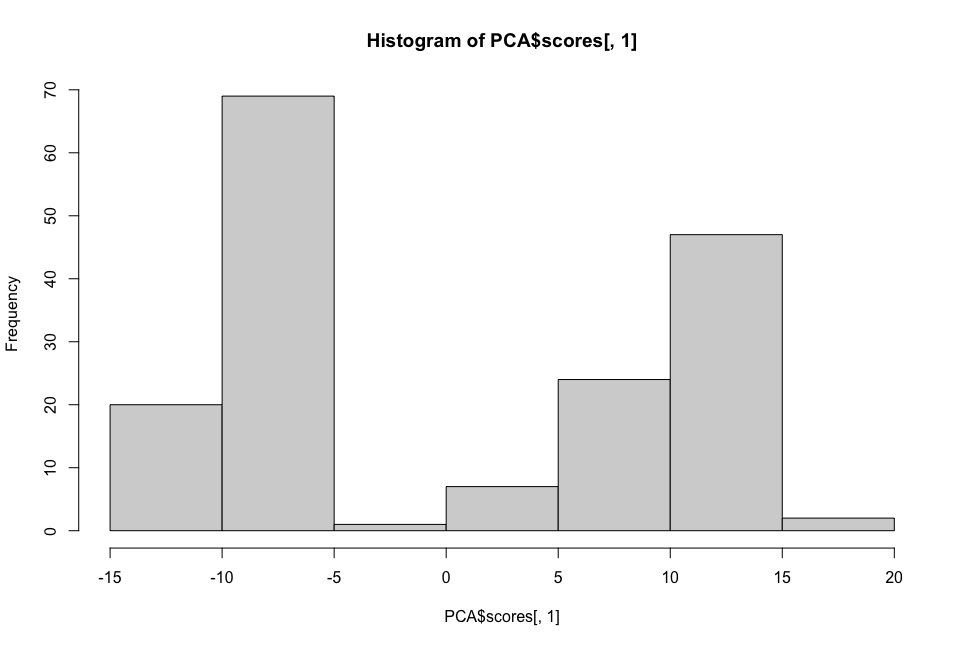
\includegraphics[width = \textwidth]{Rplot04.png}
    \end{center}
  \end{figure}
\end{exercise}

Not only can PCA reduce the dimensionality of the data significantly, but the loadings of the first component already give us a good model 
to classify the data (when we consider the scores). The loadings also tell us which survey questions we might want to question the efficacy of (questions 6 and 7). 









\end{document}


















